\section{Abstract}

\begin{singlespace}
    
The current approach used for the prediction of yields in cranberry production relies on selecting and handpicking a 300~mm~$\times$~300~mm quadrat and then extrapolating this result. In addition to being a time-consuming manual process, this system can often lead to variation in measurements due to human error as well as to spatial variation throughout the cranberry bed \cite{pozdnyakova_estimation_2002}.

This study applied machine learning algorithms in coordination with the automated image capture and detection, classification, and counting of cranberry flowers using high-resolution images. 626 genetic plots were imaged from June to August 2024 to capture peak flowering timing and were hand-annotated to create a training dataset of 1478 images with 51,732 individual annotations. These data were then used to train four machine learning models, YOLOv11, YOLOv12, Roboflow 3.0, and RF-DETR. These models were able to accurately identify, classify, and count various stages of flowering. The highest performing model, considering both accuracy and CPU latency, was YOLOv12 offering the best trade-off (mAP@0.50 = 69.3\%, F1 = 71.9\%) despite RF-DETR achieving the highest mAP.

Using this trained model, we then analyzed thirty plots. Plots were split into two groups based on genetic variation, one set of Stevens plots representing a control group and one set of Experimental variations with differing genetic traits. Plots were sampled three times at 5-day intervals from the end of June to early July, representing peak flowering timing. Using these images, we detected multiple stages of flower development and recorded flower counts per plot over the three imaging sessions. Using this new dataset, we compared the temporal flowering patterns of the two groups. Plots were also sampled in the standard method on two separate days to generate a ground truth dataset reporting fruit count and yield. Across 30 plots, total flower count moderately predicted total berry count in Experimental hybrids \rnp{0.68}{20}{= .001}.

This workflow demonstrates the potential for an automated system that can image cranberry flowers, detect and classify the blooms, and use these data to predict berry production. Although the workflow requires further development, the use of such a system would prove invaluable to growers as it enables yield signals weeks to months before harvest, informing harvest planning and in-season management.

\end{singlespace}

\section{Introduction}

Cranberry (\textit{Vaccinium macrocarpon} Ait.) is a high-value North American crop that thrives in cool, temperate climates with acidic, sandy soils and abundant freshwater sources \cite{sandler_cranberry_2008}. Wisconsin produces roughly 62\% of U.S. cranberries \cite{usda-nass_cranberries_2024}, making the crop economically and ecologically central to the state. Commercial production typically occurs in diked marshes (“bogs”) that can be flooded and drained for management and harvest; beds are constructed in low-lying areas and lined with peat, sand, and gravel to support the crop’s shallow root system. Because these engineered wetlands often occupy large, remote tracts with limited technological infrastructure, high-speed internet or even cellular coverage can be unreliable. Cranberries also require a long growing season with warm summers and cold winters to satisfy dormancy requirements \cite{ellwood_cranberry_2014}. Intensive water management—leveraging flooding for frost protection, weed control, and wet harvesting—adds operational complexity. These field conditions challenge conventional management and complicate the deployment of robotics and other precision-agriculture tools at scale. In addition to field conditions, the remote nature of most cranberry operations and connectivity constraints underscore the need for robust, field-deployable, and—ideally—edge-computing ML solutions.

Recent advances in image-based machine learning have begun to influence crop management by improving monitoring, analysis, and decision-making. In large-scale systems, ML supports crop health surveillance, weed and pest detection, yield prediction, and precision input application \cite{akiva_vision_2022}. High-resolution imagery from drones, satellites, and field cameras, paired with deep models such as convolutional neural networks (CNNs), enables early disease detection, real-time assessment, and targeted resource allocation. AI-driven weed detection improves herbicide precision \cite{wendel_self-supervised_2016}, while yield-estimation models leverage plant density, biomass, and environmental co-variates to optimize harvest planning \cite{ni_deep_2020}. Automated phenotyping accelerates breeding by quantifying traits such as berry size and shape \cite{diaz-garcia_image-based_2018}.

In specialty crops like cranberries, accurate detection of flowering stages and early fruit set is critical for yield prediction \cite{coombe_development_1980}, yet current field monitoring is labor-intensive, error-prone, and slow to deliver actionable feedback \cite{pozdnyakova_estimation_2002}. These challenges highlight the need for image-based approaches that can accommodate field variability and function reliably under real-world conditions.

This study investigates deep learning and computer vision for flower and early-fruit detection in cranberry to improve yield prediction and support precision management. Using high-resolution, ground-based imagery collected by an autonomous platform, we develop and evaluate a workflow for detection, classification, and counting. Our pipeline utilizes CNN-based architectures to accurately isolate flowers within dense canopies and address occlusion and morphological variability \cite{ghosh_understanding_2019}.

To enhance robustness, we assembled a large, annotated dataset and applied data augmentation (rotation, flipping, contrast adjustments). Beyond flower counting, we explore predictive links between floral dynamics, pollination success, and subsequent yield by integrating temporal image sequences with environmental data \cite{brown_fruit_2006,parent_current_2021}. These experiments test whether early-season imagery can forecast yield and inform irrigation, nutrition, and pollination strategies in near real-time. The novel deliverables from this project are as follows:

\par\medskip 

\begin{spacing}{1}
\begin{enumerate}[label=(\arabic*), leftmargin=2em, labelsep=0.6em, align=left,
                  itemsep=8pt, parsep=0pt, topsep=0pt, partopsep=0pt]
  \item A robust imaging platform and modeling pipeline for detecting cranberry flowers and early fruit, classifying detections, and producing counts.
  \item Creation of a dataset and training protocol designed for field variability, improving generalization across beds, cultivars, and imaging conditions.
  \item An initial demonstration that temporal flower counts correlate with early yield prediction.
\end{enumerate}
\end{spacing}

While this study focused on cranberries, the methodology could be expanded to other specialty crops that require precise floral monitoring \cite{estrada_deep_2024}.

\section{Materials and Methods}

In order to develop a high performing ML model, a large yet consistent dataset of images is required. In this study, we collected 3,308 images through manual imaging and the use of an automated ground rover at the Wisconsin Cranberry Research Station in Black River Falls, WI. The images were collected over a three month period from June 2024 to August 2024. These dates were chosen in order to capture the peak flowering dates as well as early stage fruit development \cite{sandler_cranberry_2008}. Images were collected with a Canon PowerShot A810 (Canon U.S.A, USA) with a full resolution of 4608 $\times$ 3456, giving a 16 megapixel image size. Images were captured at a height of 1500 mm and with the field of view adjusted to capture an area approximately 1200 mm $\times$ 1700 mm. This FOV and image resolution gave a ground sampling distance (GSD) of approximately 0.37 mm/px. This resolution was chosen as a typical blossom was found to be approximately 6.3 mm to 9.5 mm \cite{diaz-garcia_image-based_2018}, with some features such as individual petals being smaller. The combination of flower size and GSD ensured approximately 15-20 pixels per flower. Images were captured using natural lighting in the early afternoon to provide minimal self-shadowing and to avoid shadowing from the image collection platform. 

After images were acquired, they were cropped to a resolution of 640 $\times$ 640 px, resulting in a sample space of approximately 56,000~\(\text{mm}^2\). This size was chosen to aid in manual labeling. It was found that reducing the number of flowers to be annotated would allow annotators to more effectively visually scan the image for missing or mislabeled annotations. Reducing image size also allowed multiple samplings per image as needed to increase the number of training images. Images were also renamed at this time to add the plot number that the sample was taken from as well as the date. After pre-processing, the images were uploaded to Roboflow for annotation and training. During cropping, overlapping tiles were not used to avoid double counting, and only one image per plot/date was used.

Annotating the collected images for machine learning involved labeling images to create a training dataset used to classify features effectively\cite{ghosh_understanding_2019}. The purpose of the models in this project will be to detect flowering, classify the objects detected, and count instances of features. Relevant categories for this paper will be Early Blossoms (EB), Late Blossoms (LB) and Early Fruiting (EF). The Segment Anything Model (SAM)\cite{kirillov_segment_2023} was used to create masks and assign labels to images. SAM was used to assist annotation only; all reported results are object detection (bounding boxes), not segmentation. Special attention was given to complex scenarios, such as overlapping objects and occlusions, to ensure accurate representation. A total of 51,732 annotations were labeled across the three classes.

The full dataset was then reviewed by one annotator to ensure consistency and quality. Once validated, annotations are used to train ML models. Data were split into 70\% for training, 20\% for validation, and 10\% for testing. Additionally, splits were performed by plot and date to ensure the same plot/date never appeared in different splits, preventing near-duplicate content leakage. Our models were trained using Roboflow's NVIDIA-based GPU clusters\cite{dwyer_roboflow_2024}. Four models were used in the ML training: YOLOv11, YOLOv12\cite{jocher_ultralytics_2023}, Roboflow 3.0 (RF3), and RF-DETR\cite{deng_cross-domain_2024}.

After training, the performance was measured using mAP, Precision, Recall, and F1-score. These metrics are widely used in object detection and classification tasks to provide a comprehensive assessment of model performance\cite{rainio_evaluation_2024}.

\begin{align}
\text{Precision} &= \frac{TP}{TP+FP} \\[1ex]
\text{Recall} &= \frac{TP}{TP+FN} \\[1ex]
\text{F1-score} &= \frac{2 \times \text{Precision} \times \text{Recall}}{\text{Precision} + \text{Recall}}
\end{align}

where TP, FP, and FN denote true positives, false positives, and false negatives.

In addition to the performance benchmarks listed above, a script was created to measure inference time for the 4 selected models. The python-based script would load each model individually, run a desired number of "warm-up" inferences, and then measure the per-image inference time on a desired set of images a chosen number of times and return the results.


The best performing model was then used to analyze all images collected on a subset of plots during peak flowering season and used to produce a dataset allowing for correlation testing between flower count to yield. Yield ground truth data was gathered on two dates, with the first being on September 12\textsuperscript{th}, 2024, and the second being October 4\textsuperscript{th}, 2024. Harvest was carried out using a standard hand harvesting method of selecting a 300~mm~$\times$~300~mm quadrat and harvesting all the fruit within the boundary. After harvest, the fruit was sorted into samples of good fruit and rotten fruit by plot. Each sample was counted to determine the total number of individual fruit, identified as the Good Count (GC) and Rotten Count (RC), and then weighed to determine the yield of each sample identified as the Good Yield (GY) and Rotten Yield (RY). Thirty plots were sampled during each of the harvests, and plots were split into control plots that contained only the Stevens cultivar and Experimental plots that contained various genetic hybrids. We analyzed flower counts and ground-truth yields to quantify correlations using the SciPy library \cite{virtanen_scipy_2020} paired with the seaborn data visualization library \cite{waskom_seaborn_2021} to determine correlation between flowering timing and count to yield.


\section{Results and Discussion}

Images for training were gathered from June 14th to August 14th, 2024, at the Wisconsin Cranberry Research Station (Black River Falls, WI). Initially, a RealSense D435i (Intel, USA) camera was used; however, the resolution and lighting for the camera resulted in poor-quality images, and these images were not used. For the remainder of the season, a Canon PowerShot A810 (Canon U.S.A., USA) camera was used and provided high-quality images. The list of dates and images collected can be found in Table~\ref{tab:image dates}


\begin{table}[!ht]
    \centering
    \caption{Data Collection Dates}
    \label{tab:image dates}
    \begin{tabular}{cccc} 
      \toprule
      \textbf{Date} & \textbf{Location} & \textbf{Camera System} & \textbf{Images Collected}\\ 
      \midrule
      June 14th & East & Intel RealSense D435i & 266\\ 
      June 17th & East & Intel RealSense D435i & 266\\ 
      June 20th & East & Canon PowerShot A810 & 266\\ 
      June 21st & East & Intel RealSense D435i & 216\\ 
      June 22nd & East & Canon PowerShot A810 & 266\\ 
      June 22nd & West & Canon PowerShot A810 & 284\\
      June 27th & West & Canon PowerShot A810 & 320\\ 
      July 2nd  & East & Canon PowerShot A810 & 266\\ 
      July 2nd  & West & Canon PowerShot A810 & 360\\
      July 31st & East & Canon PowerShot A810 & 266\\ 
      Aug 5th   & East & Canon PowerShot A810 & 266\\ 
      Aug 14th  & East & Canon PowerShot A810 & 266\\
      \midrule
      \multicolumn{3}{r}{\textbf{Total}} & \textbf{3,308}\\
      \bottomrule
    \end{tabular}
\end{table}


After labeling, there were 51,732 annotated features across 1,478 images. The summary of annotation counts and average per image is shown in Table~\ref{tab:dataset-summary} with the distribution shown in Figure~\ref{fig:Annotations per Image}. For model training, the dataset was split into 1,034 training images, 297 validation images, and 147 'held-out' test images.


\begin{table}[!ht]
\centering
\caption{Dataset summary and annotation counts}
\label{tab:dataset-summary}
\footnotesize
\setlength{\tabcolsep}{6pt}

\begin{subtable}[t]{0.45\linewidth}
\centering
\caption{Annotation Counts Per Image}
\begin{tabular}{lr}
\toprule
\textbf{Metric} & \textbf{Value} \\
\midrule
Number of Images         & 1,478 \\
Mean Annotations/Image   & 35.12 \\
Standard Deviation       & 44.46 \\
\bottomrule
\end{tabular}
\end{subtable}
\hfill
\begin{subtable}[t]{0.45\linewidth}
\centering
\caption{Annotation Classes and Counts}
\begin{tabular}{lr}
\toprule
\textbf{Class} & \textbf{Count} \\
\midrule
Early Bloom (EB)  & 1,044 \\
Late Bloom (LB)   & 45,363 \\
Early Fruit (EF)  & 5,325 \\
\midrule
\textbf{Total}    & \textbf{51,732} \\
\bottomrule
\end{tabular}
\end{subtable}
\end{table}



\begin{figure}[!ht]
    \centering
    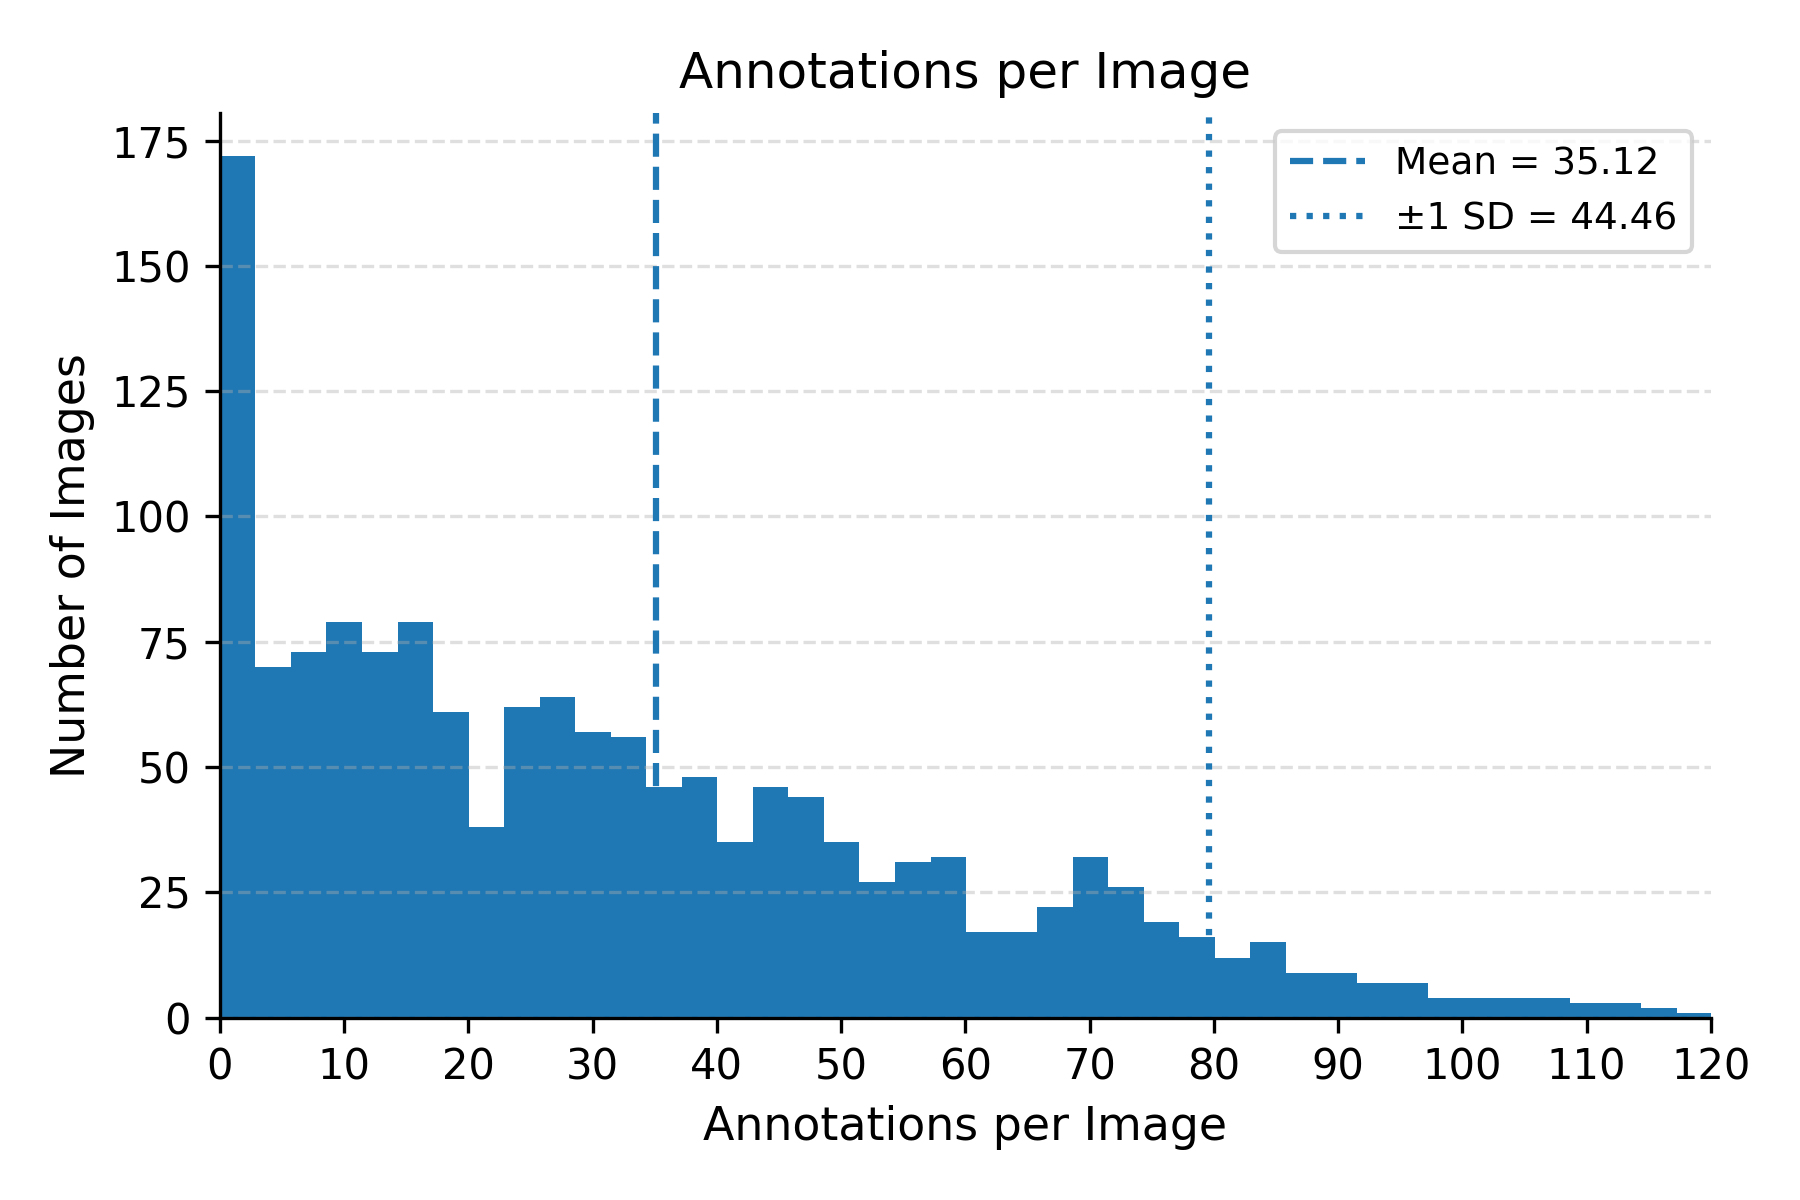
\includegraphics[width=0.75\linewidth]{images/Annotations per Image.png}
    \caption{Distribution of per–image annotation counts across the labeled dataset used to train the detectors. With a mean of 32 annotations per image with a wide standard deviation.}

    \label{fig:Annotations per Image}
\end{figure}

% -- Remove to simplify --
% Possibly due to the timing of the data collection, a majority of the blooms captured were of the late bloom stage. The timing that a flower would stay at the early stage bloom appeared to last for less than 24 hours, resulting in only a small amount of flowers actually being captured in this stage. After these flowers were open, they would remain intact on the uprights through multiple imaging sessions.

Due to the low number of early bloom flowers noted, they were merged into the larger group of total flower count that included all bloomed flowers regardless of stage.

\begin{equation}
\label{eq:TFC}
\text{Total Flower Count} = {\text{EB + LB}}
\end{equation}
\vspace{10pt}

An example of an annotated image with both Early and Late Blooms can be seen in Figure~\ref{fig:early and late bloom}

\begin{figure}[H]
    \centering
    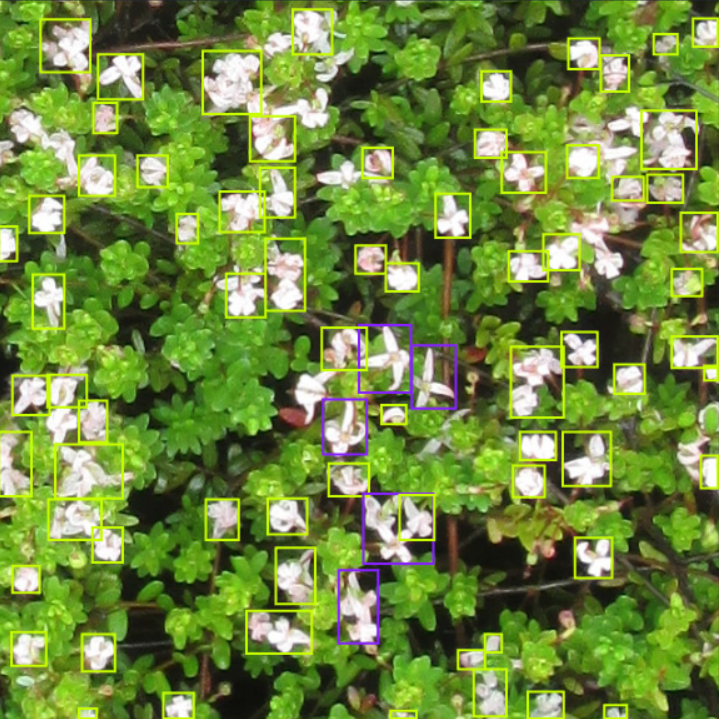
\includegraphics[width=0.5\linewidth]{images/Early and Late Bloom.png}
    \caption{Example annotated frame showing both Early Bloom (EB) and Late Bloom (LB) classes. Colored boxes indicate model targets; EB+LB defines the Total Flower Count used throughout the analysis. This illustration clarifies stage definitions and shows typical occlusion/lighting conditions encountered in the field.}
    \label{fig:early and late bloom}
\end{figure}

Both YOLO models and RF3 were trained to 150 epochs and the RF-DETR model was trained to 25 epochs. These training times are in line with current results as YOLO models often benefit from longer schedules due to heavy stochastic augmentation where longer schedules yield new views of the data and steady AP gains \cite{bochkovskiy_yolov4_2020}. In contrast, modern DETR-style models that RF-DETR builds on adopt architectural and training tweaks that accelerate convergence compared with the original DETR \cite{zhu_deformable_2021}. However, the original DETR needed ~500 epochs on COCO, whereas DINO reports competitive accuracy in just 12–24 epochs \cite{wang_rt-detrv3_2025}.

After training, the performance of each model is shown below in Table~\ref{tab:model-performance-comparison}. On the held-out test set, RF-DETR achieved the most accurate results with mAP@0.50 = 74.2\%, Precision = 77.0\%, Recall = 70.2\%; YOLOv12 performed the highest among the YOLO family of models tested and achieved mAP@0.50 = 69.3\%, Precision = 79.0\%, Recall = 66.4\%. The results for the time to inference test are also shown in Table~\ref{tab:inference time}. The inference time between v11, v12, and RF3 was very close, with v11 being slightly quicker as expected, and RF-DETR had significantly higher latency \cite{gonzalez_hernandez_analysis_2025}\cite{saltik_comparative_2025}.  

\begin{table}[!ht]
\centering
\caption{Model Performance Comparison}
\label{tab:model-performance-comparison}
\footnotesize
\setlength{\tabcolsep}{6pt}
\begin{tabular}{ccccc}
\toprule
\textbf{Model} & \textbf{mAP@50 (\%)} & \textbf{Precision (\%)} & \textbf{Recall (\%)} & \textbf{F1-Score (\%)} \\
\midrule
YOLOv11  & 67.1 & 68.7 & 71.6 & 70.1 \\
YOLOv12  & 69.3 & 79.0 & 66.4 & 71.9 \\
RF3      & 65.9 & 76.7 & 65.8 & 70.6 \\
RF-DETR  & 74.2 & 77.0 & 70.2 & 73.2 \\
\bottomrule
\end{tabular}
\end{table}

Comparing the models directly, RF-DETR favors global reasoning and end-to-end simplicity, YOLOv12 injects stronger attention for context while aiming to stay real-time, YOLOv11 maximizes efficiency within the classic convolutional recipe, and Roboflow 3 emphasizes ease of deployment. Based on this, we can select based on priority of accuracy/segmentation (RF-DETR), attention-driven context at speed (v12), edge-friendly throughput (v11), or smooth training-to-deployment workflows with flexible latency/accuracy trade-offs (RF3).


 We measured CPU inference latency on a Dell Precision 5550 (Intel i7-10850H, 64 GB RAM) with batch size = 1, input = 640$\times$640, 5 warm-up runs, and 25 timed runs per model, reporting average/median/P95 per-image latency in Table~\ref{tab:inference time}.

\begin{table}[!ht]
\centering
\caption{CPU Inference Time Summary}
\label{tab:inference time}
\footnotesize
\setlength{\tabcolsep}{6pt}
\begin{tabular}{ccccc}
\toprule
\textbf{Model} & \textbf{Timed Runs (N)} & \textbf{Avg Latency (ms)} & \textbf{Median (ms)} & \textbf{P95 (ms)} \\
\midrule
YOLOv12 & 25 & 205.98 & 212.60 & 223.72 \\
YOLOv11 & 25 & 184.17 & 183.88 & 205.26 \\
RF3 & 25 & 196.07 & 195.73 & 211.46 \\
RF-DETR & 25 & 683.50 & 682.44 & 724.35 \\
\bottomrule
\end{tabular}
\end{table}


This performance is found to be in line with current findings comparing these models \cite{kumar_container_2025}. Considering that all the models tested are state-of-the-art models and are typically built upon previous versions, the similarity in results is expected. Similar to relevant studies that have seen improvement \cite{yang_gtdr-yolov12_2025}, we also saw increased performance of YOLOv12 over YOLOv11. Recent work in blueberry breeding has demonstrated the use of YOLOv11-based pipelines to classify fruit maturity and provide a proxy for yield estimation, highlighting the potential of object detection frameworks for small fruit crops \cite{zhang_open-source_2024,li_high-throughput_2025}.

After the successful creation of the ML model, we used the YOLOv12 model to analyze thirty plots for yield correlation. Although RF-DETR achieved the highest mAP@0.50 (74.2\%), YOLOv12’s mAP was within 4.9 points, and the median CPU latency was 3.2$\times$ lower than RF-DETR at 640×640 (213 ms vs 682 ms). Due to the significant difference in inference time compared to mAP, we employed YOLOv12 for downstream plot analysis.  Plots were split into two groups based on genetic variation, one set of Stevens cultivar representing a control group and one set of Experimental variations with differing genetic traits. Plots were sampled three times at 5-day intervals from the end of June to early July, representing peak flowering timing. Using these images, we detected multiple stages of flower development and recorded flower counts per plot over the three imaging sessions. Using this new dataset, we compared the temporal flowering patterns of the two groups. The data collected is shown in Table~\ref{tab: Flower Count Data}. Plotting this data by group, we see a trend of decreasing flower count by date. It is also notable that the Stevens cultivar has less variability in flower count over time. 

%==================== Table B: Flower Counts ====================
\begin{table}[!ht]
\centering
\caption{Collected Data — Flower Counts}
\label{tab: Flower Count Data}
\footnotesize
\setlength{\tabcolsep}{4pt}
\adjustbox{max width=\textwidth}{%
\begin{tabular}{ccccc}
\toprule
\textbf{Plot Number} & \textbf{Type} & \textbf{22-June} & \textbf{27-June} & \textbf{2-July} \\
\midrule
1  & Experimental & 212 & 29  & 31  \\
2  & Experimental & 163 & 31  & 112 \\
3  & Stevens      & 186 & 104 & 43  \\
4  & Stevens      & 181 & 174 & 34  \\
5  & Stevens      & 147 & 47  & 34  \\
6  & Experimental & 125 & 123 & 92  \\
7  & Stevens      & 248 & 105 & 44  \\
8  & Experimental & 118 & 52  & 51  \\
9  & Stevens      & 207 & 139 & 13  \\
10 & Stevens      & 172 & 100 & 47  \\
11 & Experimental & 165 & 120 & 78  \\
12 & Stevens      & 206 & 86  & 44  \\
13 & Experimental & 130 & 78  & 47  \\
14 & Experimental & 95  & 83  & 21  \\
15 & Experimental & 237 & 229 & 41  \\
16 & Stevens      & 184 & 38  & 24  \\
17 & Experimental & 143 & 172 & 60  \\
18 & Experimental & 256 & 101 & 117 \\
19 & Experimental & 135 & 98  & 74  \\
20 & Experimental & 98  & 36  & 50  \\
21 & Stevens      & 110 & 69  & 28  \\
22 & Experimental & 208 & 256 & 158 \\
23 & Experimental & 206 & 60  & 87  \\
24 & Experimental & 102 & 105 & 53  \\
25 & Experimental & 162 & 39  & 36  \\
26 & Experimental & 120 & 104 & 17  \\
27 & Experimental & 185 & 96  & 72  \\
28 & Experimental & 85  & 95  & 78  \\
29 & Stevens      & 106 & 51  & 26  \\
30 & Experimental & 100 & 102 & 67  \\
\midrule
\textbf{Experimental Mean} &  & \textbf{152} & \textbf{100} & \textbf{67} \\
\textbf{Experimental Std}  &  & \textbf{51}  & \textbf{60}  & \textbf{35} \\
\textbf{Stevens Mean}      &  & \textbf{175} & \textbf{91}  & \textbf{34} \\
\textbf{Stevens Std}       &  & \textbf{44}  & \textbf{43}  & \textbf{11} \\
\bottomrule
\end{tabular}}
\end{table}


\begin{figure}[H]
    \centering
    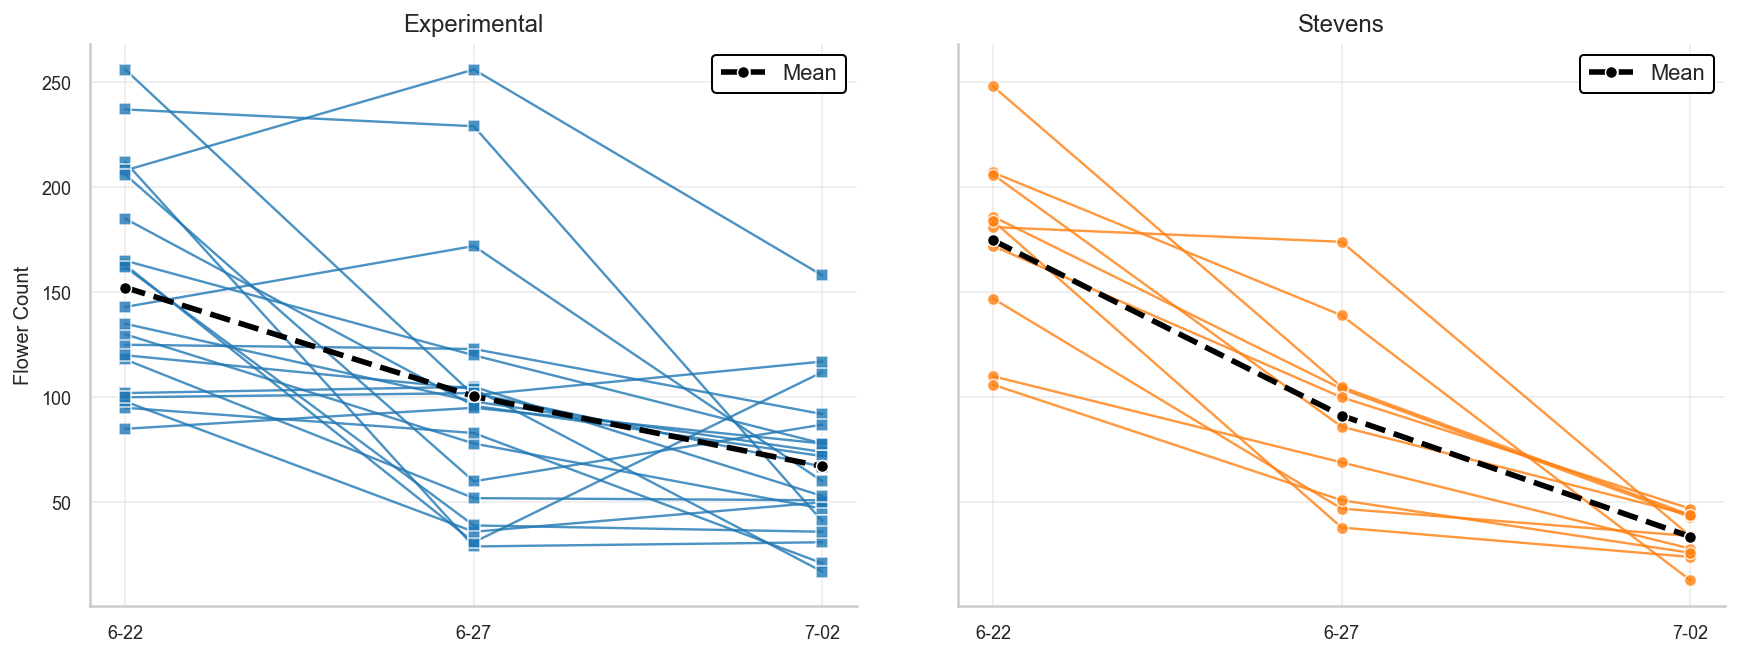
\includegraphics[width=0.85\linewidth]{images/Count by Type vs Date.png}
    \caption{Flower count by date, stratified by cultivar type (Stevens vs Experimental). Points are plot-level observations across three imaging sessions; the line traces the date-wise mean, highlighting bloom rise and peak timing by cohort. This view supports later yield analyses by establishing the temporal context of flowering intensity.}
    \label{fig:Count by Type vs Date}
\end{figure}

At the completion of the growing season, plots were sampled in the standard method of collecting all berries in a 300~mm~$\times$~300~mm quadrat on two separate days to generate a ground truth dataset. This data was recorded as fruit count and yield. This data is shown in Table~\ref{tab: Harvest Data}

%==================== Table A: Harvest 1 & Harvest 2 ====================
\begin{table}[!ht]
\centering
\caption{Collected Data — Harvest 1 and Harvest 2}
\label{tab: Harvest Data}
\footnotesize
\setlength{\tabcolsep}{4pt}
\adjustbox{max width=\textwidth}{%
\begin{tabular}{|c|c|c|c|c|c|c|c|c|c|}
\cline{3-10}
\multicolumn{1}{c}{} & \multicolumn{1}{c}{} & \multicolumn{4}{|c|}{Harvest 1} & \multicolumn{4}{c|}{Harvest 2} \\
\hline{}
\multirow{2}{*}{Plot Number} & \multirow{2}{*}{Type} & Good Count & Rotten Count & Good Yield & Rotten Yield & Good Count & Rotten Count & Good Yield & Rotten Yield \\
 &  & \textit{(Number of Berries)} & \textit{(Number of Berries)} & \textit{(g)} & \textit{(g)} & \textit{(Number of Berries)} & \textit{(Number of Berries)} & \textit{(g)} & \textit{(g)} \\
\hline
1 & Experimental & 232 & 32 & 315.1 & 41.4 & 131 & 15 & 199.7 & 15.6 \\
2 & Experimental & 125 & 63 & 172.0 & 63.0 & 54 & 36 & 81.6 & 47.3 \\
3 & Stevens      & 70  & 28 & 138.4 & 41.9 & 30  & 23 & 66.2 & 35.6 \\
4 & Stevens      & 49  & 19 & 80.5  & 22.3 & 39  & 47 & 84.4 & 78.2 \\
5 & Stevens      & 134 & 9  & 293.5 & 15.4 & 99  & 28 & 217.6 & 49.0 \\
6 & Experimental & 126 & 47 & 148.3 & 48.7 & 72  & 33 & 84.9 & 34.9 \\
7 & Stevens      & 60  & 38 & 117.8 & 62.8 & 89  & 138 & 186.7 & 228.5 \\
8 & Experimental & 90  & 48 & 116.4 & 50.9 & 95  & 120 & 145.6 & 143.7 \\
9 & Stevens      & 79  & 32 & 171.3 & 49.5 & 89  & 91 & 199.7 & 151.8 \\
10 & Stevens     & 139 & 38 & 258.0 & 67.3 & 67  & 26 & 145.8 & 40.0 \\
11 & Experimental & 143 & 35 & 219.6 & 40.9 & 33  & 57 & 59.9 & 81.8 \\
12 & Stevens     & 111 & 51 & 197.8 & 77.6 & 59  & 59 & 110.2 & 99.4 \\
13 & Experimental & 137 & 18 & 179.6 & 22.5 & 50  & 79 & 80.0 & 92.4 \\
14 & Experimental & 134 & 24 & 181.8 & 25.5 & 60  & 28 & 105.1 & 36.0 \\
15 & Experimental & 276 & 52 & 188.5 & 29.3 & 174 & 44 & 142.3 & 30.2 \\
16 & Stevens     & 78  & 13 & 140.5 & 17.3 & 31  & 7  & 62.3 & 12.5 \\
17 & Experimental & 108 & 121 & 108.6 & 106.3 & 39 & 94 & 41.9 & 99.4 \\
18 & Experimental & 97  & 84 & 121.2 & 92.6 & 59  & 98 & 84.7 & 111.6 \\
19 & Experimental & 129 & 5  & 153.5 & 4.3 & 132 & 11 & 176.0 & 14.1 \\
20 & Experimental & 148 & 20 & 174.8 & 21.2 & 92  & 94 & 140.8 & 112.3 \\
21 & Stevens     & 55  & 3  & 127.9 & 2.9 & 70  & 24 & 157.4 & 52.9 \\
22 & Experimental & 297 & 3  & 170.0 & 1.7 & 246 & 16 & 155.3 & 9.7 \\
23 & Experimental & 127 & 19 & 162.0 & 19.4 & 124 & 50 & 155.2 & 61.2 \\
24 & Experimental & 120 & 15 & 152.7 & 15.0 & 94  & 85 & 137.7 & 101.1 \\
25 & Experimental & 113 & 94 & 137.5 & 75.2 & 102 & 64 & 138.6 & 69.6 \\
26 & Experimental & 82  & 62 & 97.9  & 61.0 & 42  & 62 & 55.7 & 74.9 \\
27 & Experimental & 207 & 22 & 164.4 & 15.8 & 190 & 47 & 143.3 & 35.3 \\
28 & Experimental & 86  & 66 & 114.8 & 70.9 & 36  & 142 & 53.6 & 166.5 \\
29 & Stevens     & 99  & 15 & 211.9 & 19.7 & 89  & 35 & 186.6 & 59.2 \\
30 & Experimental & 140 & 27 & 169.6 & 27.0 & 64  & 36 & 86.7 & 34.2 \\
\hline
\rowcolor{lightgray} Experimental Mean &  & \textbf{146} & \textbf{43} & \textbf{162.4} & \textbf{41.6} & \textbf{94} & \textbf{42} & \textbf{113.4} & \textbf{68.6} \\
\rowcolor{lightgray} Experimental Std  &  & \textbf{60}  & \textbf{31} & \textbf{47.3}  & \textbf{29.0} & \textbf{57} & \textbf{29} & \textbf{45.3}  & \textbf{44.4} \\
\rowcolor{lightgray} Stevens Mean      &  & \textbf{87}  & \textbf{25} & \textbf{173.8} & \textbf{37.7} & \textbf{66} & \textbf{38} & \textbf{141.7} & \textbf{80.7} \\
\rowcolor{lightgray} Stevens Std       &  & \textbf{32}  & \textbf{15} & \textbf{66.5}  & \textbf{25.7} & \textbf{26} & \textbf{26} & \textbf{57.5}  & \textbf{64.8} \\
\hline
\end{tabular}}
\end{table}


Due to a relatively low sample size of both Stevens and Experimental plots, 10 plots and 20 plots respectively, it was decided to also consider the total berry count of both harvests and total flower count from all sessions as an additional dataset. 

\begin{figure}[!ht]
  \begin{subfigure}{0.45\textwidth}
    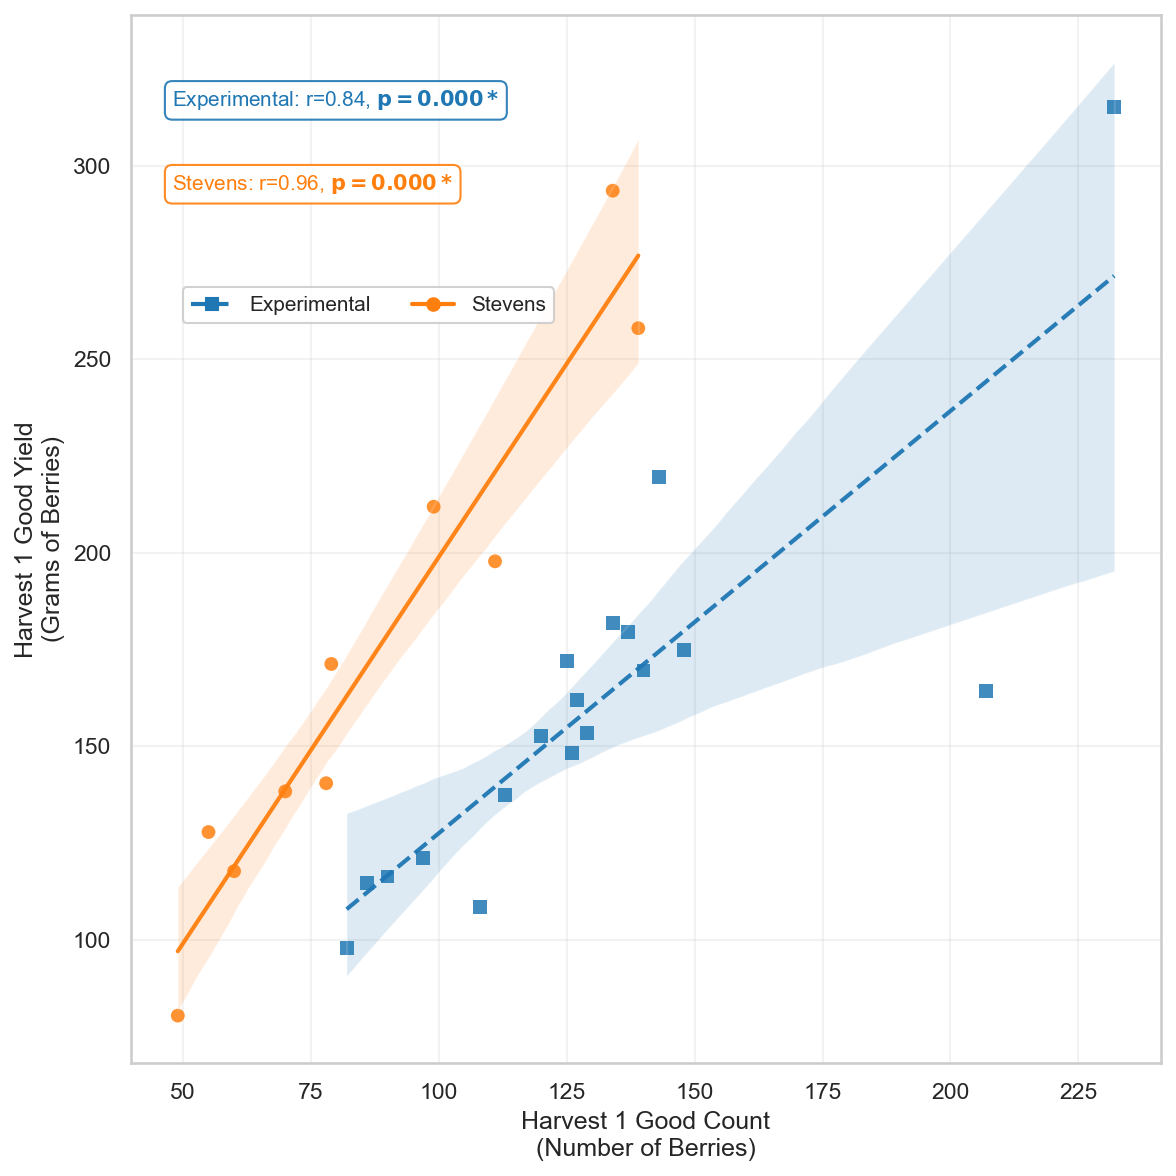
\includegraphics[width=\textwidth]{images/h1-countvsyield.png}
   \caption{Harvest 1 Count vs Yield}
    \label{fig:H1 Count vs Yield}
  \end{subfigure}
  \hfill
  \begin{subfigure}{0.45\textwidth}
    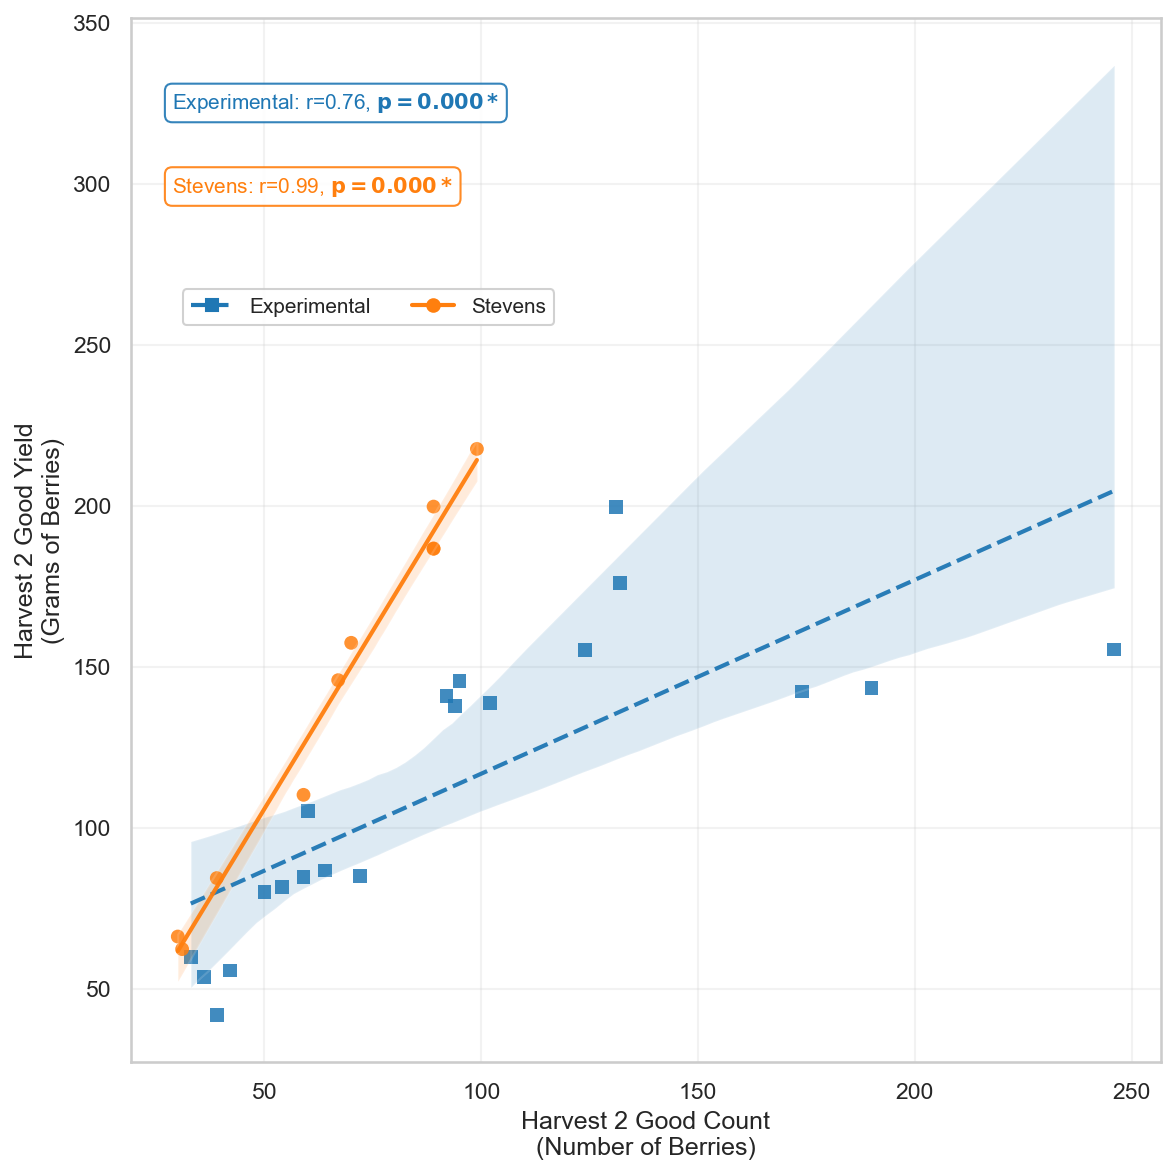
\includegraphics[width=\textwidth]{images/h2-countvsyield.png}
   \caption{Harvest 2 Count vs Yield}
    \label{fig:H2 count to yield}
  \end{subfigure}
  \caption{Relationship between plot-level berry count and measured yield for (a) Harvest 1 and (b) Harvest 2. Lines show ordinary least squares (OLS) fits; shaded bands are 95\% confidence intervals. Strong positive associations across both harvests justify using berry counts as a proxy for yield and provide a baseline for linking early flowering to end-of-season outcomes.}
  \label{fig:Harvest count comparison}
\end{figure}

 Pearson’s r (two-tailed p) was computed with SciPy \cite{virtanen_scipy_2020} and visualized with seaborn.\cite{waskom_seaborn_2021} The Pearson’s correlation coefficient (r) quantifies the strength and direction of the linear association between two continuous variables by standardizing their covariance. We used Pearson's r with two-tailed p-values to summarize pairwise relationships, noting it captures linear dependence\cite{sedgwick_pearsons_2012}.

 In order to ensure a robust relationship between flower count and yield, the correlation between harvest counts and yield was first needed. Figure~\ref{fig:Harvest count comparison} shows a strong correlation between berry count and yield of the Experimental cultivar in both Harvest 1 and Harvest 2, \rnp{0.76}{20}{<.001} and \rnp{0.84}{20}{<.001} respectively. This trend was also seen in the Stevens cultivar, with the correlation between berry count and yield in Harvest 1 and Harvest 2 being \rnp{0.96}{10}{<.001} and \rnp{0.99}{10}{<.001}. This mirrors work in blueberries demonstrating that berry number is the primary driver of yield and can serve as a reliable predictor \cite{salvo_estimate_2012,percival_narrow_2012}. Additionally, this correlation shows a consistency of berry mass and distinctly a greater consistency in the Stevens plots, which is expected as these plots have reduced genetic diversity and more consistent fruit sizing \cite{gallardo_breeding_2018}.


Next, the correlation between flower count and berry count was investigated. Due to the high number of datasets consisting of three flowering dates, a total flower count, in addition to two harvest dates and their totals, a pair plot was used to find relevant correlation, as shown in Figure~\ref{fig:Flower Pair-Plot} found in the Appendix. 


\begin{figure}[!ht]
  \begin{subfigure}{0.45\textwidth}
    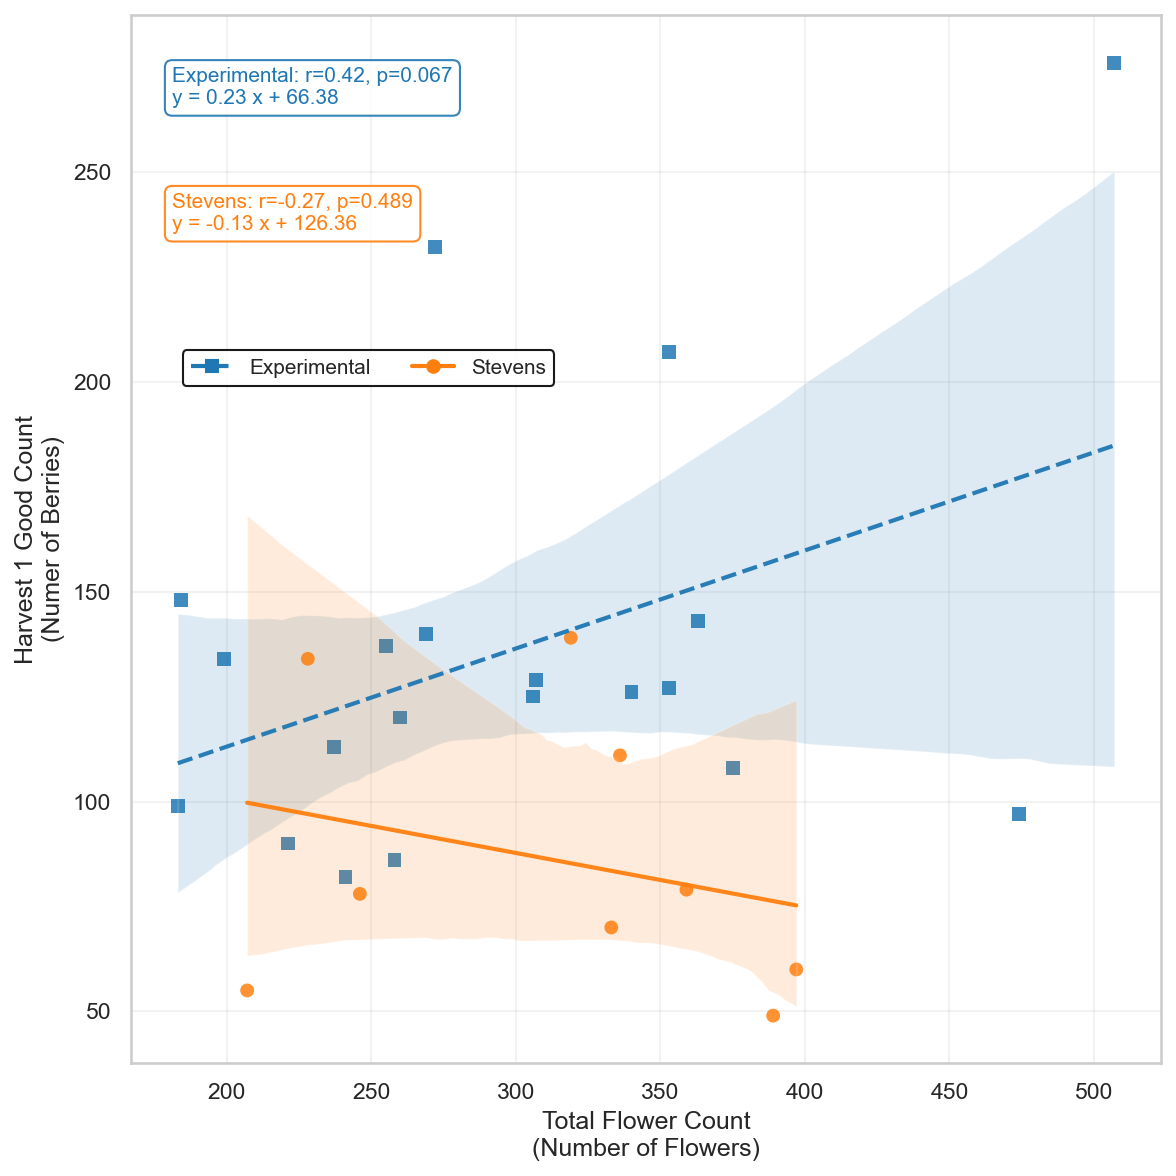
\includegraphics[width=\textwidth]{images/H1 GC vs TFC.png}
   \caption{Harvest 1 Good Count vs Total Flower Count}
    \label{fig:H1 GC vs TFC}
  \end{subfigure}
  \hfill
  \begin{subfigure}{0.45\textwidth}
    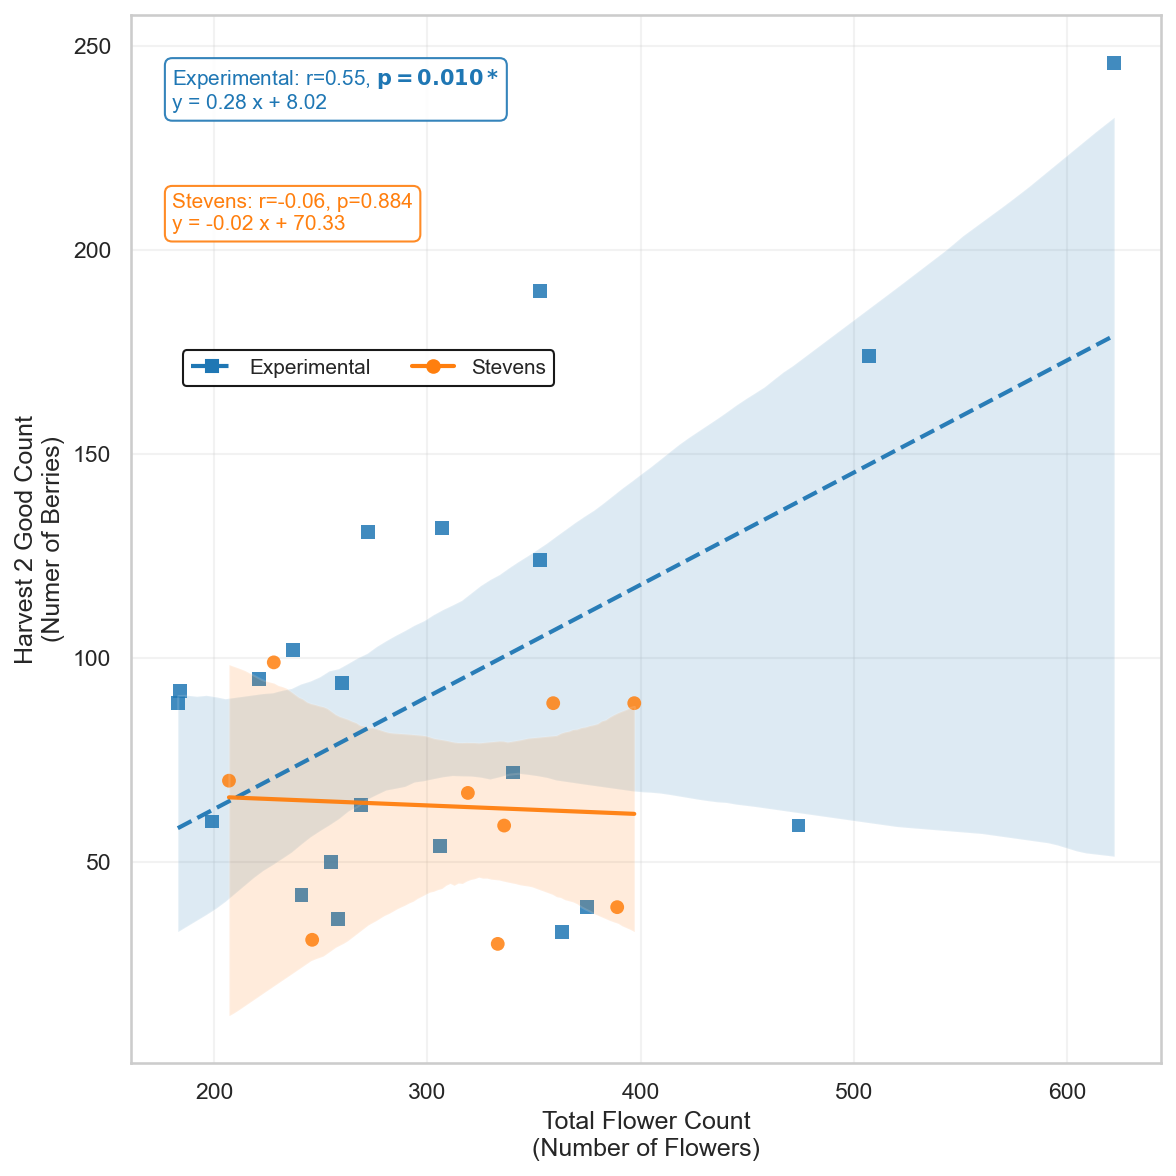
\includegraphics[width=\textwidth]{images/H2 GC vs TFC.png}
   \caption{Harvest 2 Good Count vs Total Flower Count}
    \label{fig:H2 GC vs TFC}
  \end{subfigure}
  \caption{Good berry count at (a) Harvest 1 and (b) Harvest 2 versus Total Flower Count (sum of Early + Late blooms). Points are plot-level values by cultivar; OLS lines with 95\% confidence bands summarize the trend. Experimental hybrids show a moderate to significant association, while Stevens differs, motivating cultivar-specific interpretation of flower-to-fruit conversion and possible variation in ripening dynamics.}
  \label{fig:GC vs TFC}
\end{figure}


When comparing flower counts to good berry count, however, results were more nuanced as seen in Figure~\ref{fig:GC vs TFC}. Experimental hybrids showed a moderate but significant correlation between total flower count and good berry count \rnp{0.55}{20}{= .010}. Stevens, in contrast, exhibited stronger correlations between total flower count and rotten berry count \rnp{0.70}{10}{= .034} as seen in Figure~\ref{fig:RC vs TFC}. This divergence may reflect cultivar-specific ripening dynamics, with Stevens plots appearing to have fruit overripen before harvest, resulting in higher rot incidence, while Experimental hybrids were closer to peak ripening at the time of collection. Some cultivar-dependent differences in flower-to-fruit conversion efficiency and fruit quality outcomes have been documented in blueberry production \cite{cortes-rivas_pollination_2023} and differences in fruit quality outcomes—such as berry size, mass, color, and biochemistry—have been well documented in cranberry breeding populations \cite{loarca_berryportraits_2024,maule_buds_2024}.

\begin{figure}[!ht]
  \begin{subfigure}{0.5\textwidth}
    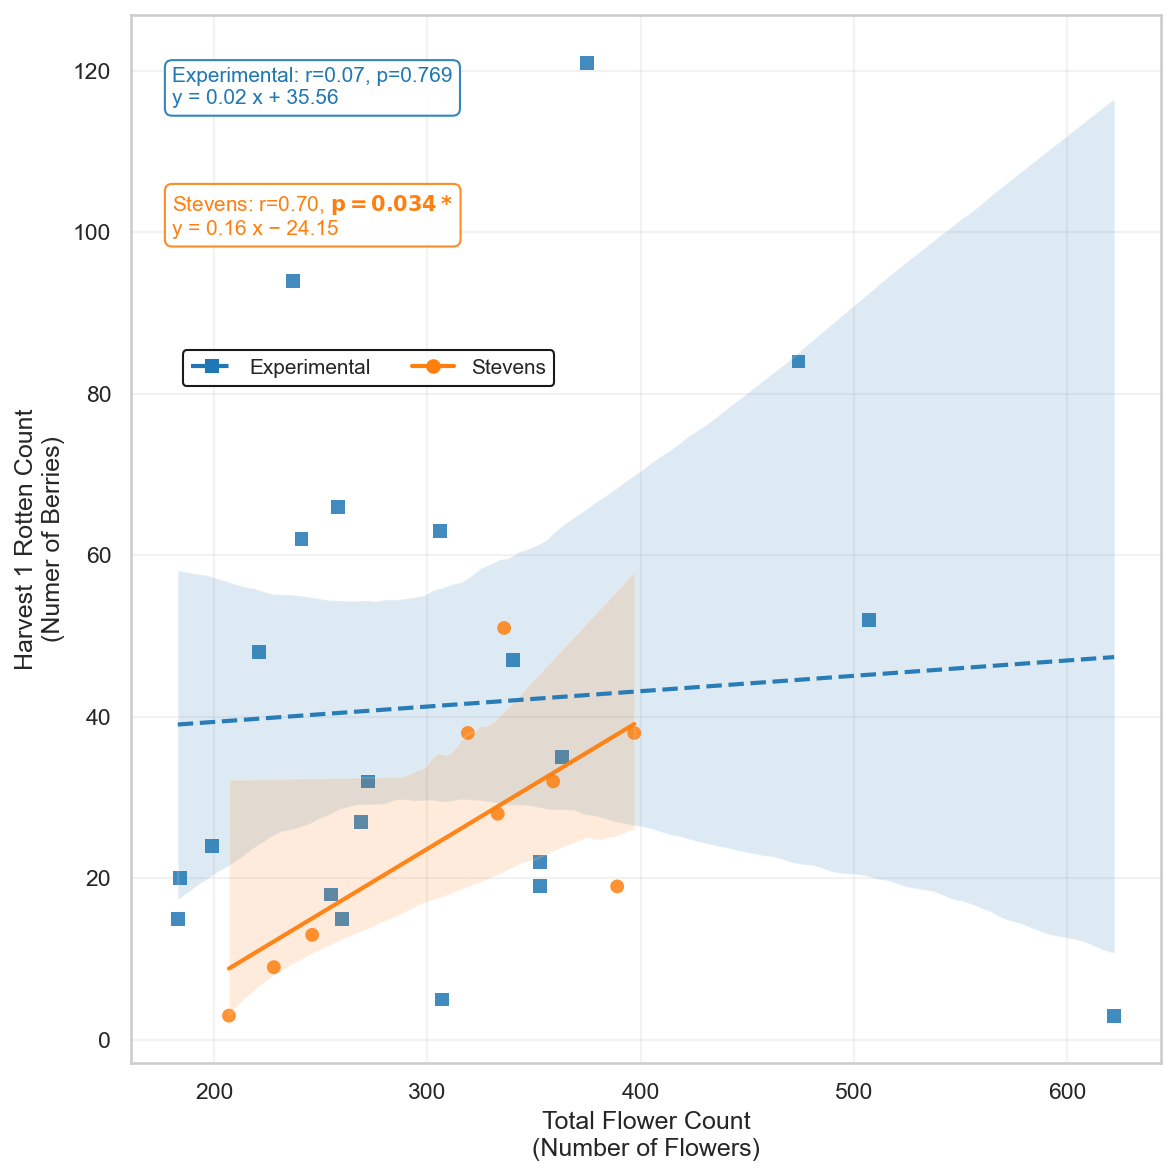
\includegraphics[width=\textwidth]{images/H1 RC vs TFC.png}
   \caption{Harvest 1 Rotten Count vs Total Flower Count}
    \label{fig:H1 RC vs TFC}
  \end{subfigure}
  \hfill
  \begin{subfigure}{0.5\textwidth}
    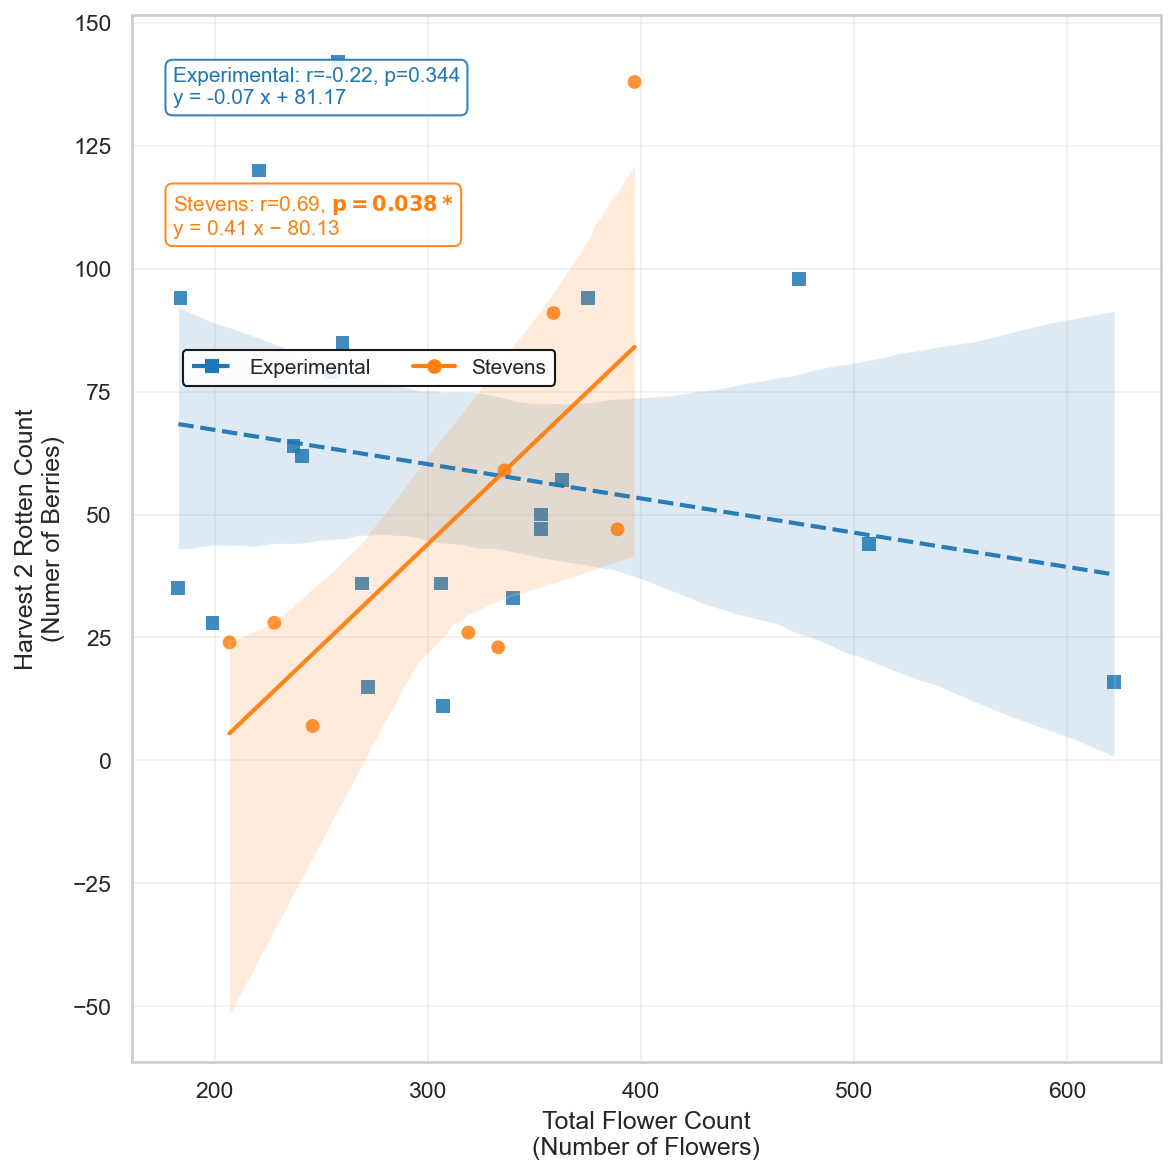
\includegraphics[width=\textwidth]{images/H2 RC vs TFC.png}
   \caption{Harvest 2 Rotten Count vs Total Flower Count}
    \label{fig:H2 RC vs TFC}
  \end{subfigure}
  \caption{Rotten berry count at (a) Harvest 1 and (b) Harvest 2 versus Total Flower Count. OLS fits with 95\% CIs reveal a stronger positive association for Stevens than for Experimental hybrids, likely due to cultivar-dependent ripening dynamics and post-set losses that raise rot incidence in Stevens under the season’s conditions.}
  \label{fig:RC vs TFC}
\end{figure}

In Figure~\ref{fig:TBC vs TFC}, total flower count is positively associated with total berry count. The relationship is moderate and statistically significant in the Experimental hybrids \rnp{0.68}{20}{= .001}, but weaker and not significant in Stevens \rnp{0.39}{10}{= .304}. This divergence is consistent with cultivar-specific dynamics noted earlier (e.g., greater post-set losses/rot in Stevens), indicating that flower abundance provides a more reliable early yield signal in the Experimental cohort under this season’s conditions. Practically, plots with more flowers tended to produce more berries, supporting flower counts as a viable, image-based proxy for eventual berry set.


\begin{figure}[H]
    \centering
    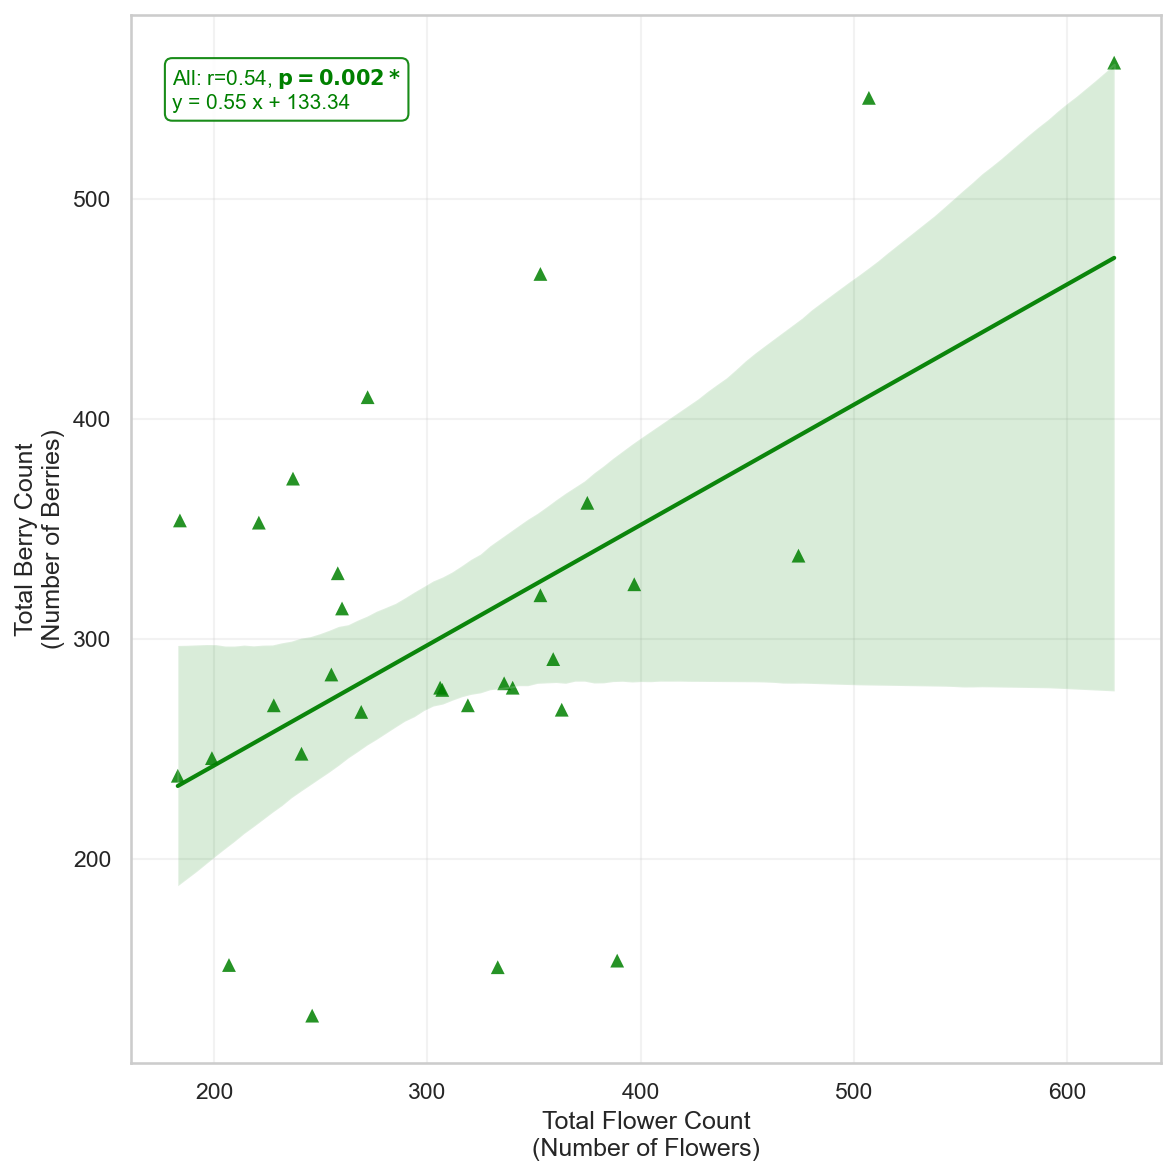
\includegraphics[width=0.75\linewidth]{images/TBC to TFC all Cultivars.png}
    \caption{Total Berry Count (both harvests combined) versus Total Flower Count aggregated over the standardized bloom window. Each point is a plot; the OLS fit with 95\% CI shows a clear, positive relationship overall and a stronger signal in the Experimental cultivars. This supports using early flower abundance as an image-based indicator of expected berry number under similar conditions.}
    \label{fig:TBC vs TFC APT}
\end{figure}

\begin{figure}[H]
    \centering
    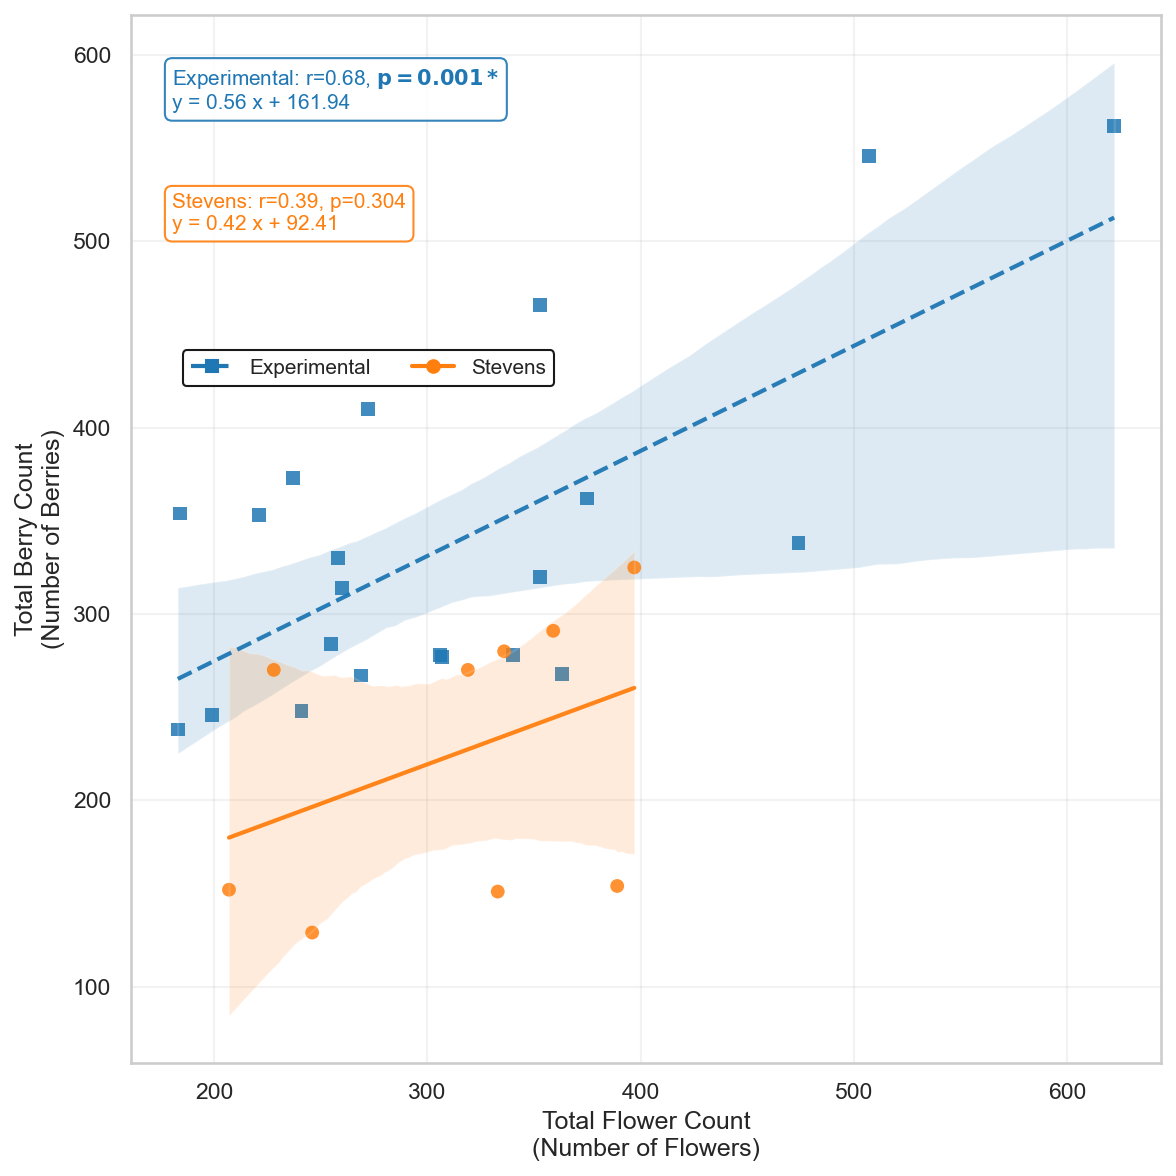
\includegraphics[width=0.75\linewidth]{images/TBC vs TFC.png}
    \caption{Total Berry Count across all harvests and cultivars versus Total Flower Count over the bloom window with no distinction between cultivar types. the OLS fit with 95\% CI shows a clear, positive relationship overall and a strong correlation. This supports using early flower abundance as an image-based indicator of expected berry number under similar conditions.}
    \label{fig:TBC vs TFC}
\end{figure}


\section{Conclusion}
We demonstrated an end-to-end workflow from ground image capture, assisted annotation, and object-detection modeling—that is then able to detect and count cranberry flowers to be used to predict berry count. Among four modern detectors, YOLOv12 offered the best accuracy/latency trade-off for edge deployment (mAP@0.50 = 69.3\%, F1 = 71.9\%), with inference latency $\approx$3.2$\times$ lower than RF-DETR at 640$\times$640. We then used the YOLOv11 model to quantify relationships between flowering and harvest outcomes across 30 plots. Total flower count moderately predicted total berry count in Experimental hybrids \rnp{0.68}{20}{= .001}, while cultivar-specific ripening patterns likely contributed to the stronger association between flowers and rot in Stevens. 

These findings suggest that low-cost cameras combined with on-device inference can provide growers with useful yield estimates several weeks before harvest. Compared with manual quadrat sampling, automated imaging increases spatial coverage and temporal frequency, improving robustness to within-bed variability. 

Future work should refine class definitions, establish standardized imaging schedules to distinguish pollination success from post-set fruit loss, and increase imaging frequency to improve predictive accuracy. A larger, multi-site study with standardized imaging windows and pre-specified analyses will help translate these early correlations into calibrated, cultivar-aware yield predictors suitable for commercial adoption.

\section{References}

\printbibliography[heading=none]